\section{Dense Ordinary Neural Networks}
\subsection{A Study of the Number of Parameters in a Network}
In previous sections I have discussed the reasoning for not wanting an automated process for building network architectures (otherwise known
as hyperparameter searches). Although, I found manually choosing the architecture for each model to be preferable in this analysis, there 
are some downsides to that decision. When building each model I wanted to ensure that the performances of said models were representative of 
the category of models I wanted to build. In other words, I wanted to ensure that any drawbacks were related to the type of model (i.e. \ac{LWTA}, \ac{PNN} etc.) 
and not a result of poorly chosen number of layers or nodes. Therefore, I wanted to remove as much subjectivity in the choice of architecture as possible.
\\
In this section I present a comparison of the results from two ordinary dense \ac{NN} with different amount of nodes. The first network 
uses the dense \ac{NN} architecture described in \ref{subsec:arch} and illustrated in figure \ref{fig:arch}, while the second network uses the same activation 
functions and amount of hidden layers, but with only 20 nodes in each layer. The comparison presented in this thesis represent a sample of networks I choose to 
compare when deciding the number of nodes and hidden layers to be used in the analysis. Both networks apply the training strategy described in section 
\ref{subsec:TrainingStrategy}.
\\
Figure \ref{fig:NNshallowGridSig} displays the expected sensitivity for the smaller network (20 nodes). By comparing with the 
results achieved by the \verb!XGBoost! model in figure \ref{fig:XGBoost}, we can observe that the shallow network performs very similarly to the \verb!XGBoost! 
model. In fact, the \verb!XGBoost! model seems to outperform (achieve a higher significance for most combinations) the network ever so slightly.
\\
In figure \ref{fig:NNGridSig}, I present the same grid as described above, but using the larger network. By comparing the results from the smaller 
network in figure \ref{fig:NNshallowGridSig}, we can discern that the larger network outperforms the smaller network for every single mass 
combination in the original signal set. The higher the number of nodes and layers, the more parameters need tuning during training, 
and consequently the more data is needed during training. Generally, the more complex the problem, the more parameters are needed in a model. Therefore, 
based on the comparison between the two networks, we can draw the conclusion that the data used in this analysis is enough to tune a relatively 
deep network with large amount of parameters. This result motivated the choice of layers and nodes for all networks used in the sections to come.
\begin{figure}
    \makebox[\linewidth][c]{%
    \centering
    \begin{subfigure}{.6\textwidth}
        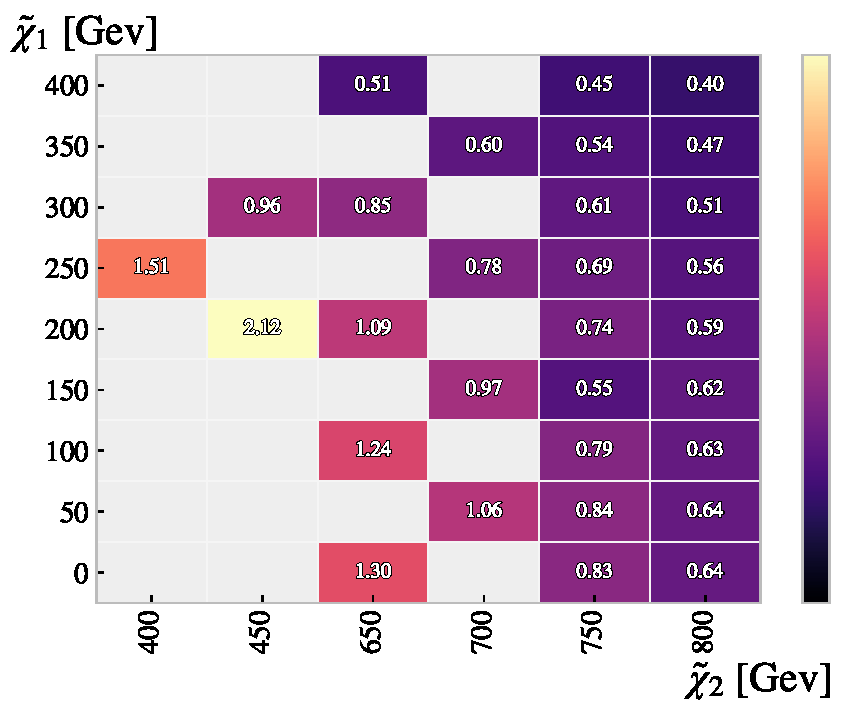
\includegraphics[width=\textwidth]{Figures/MLResults/NN/SUSY/Grid/NNshallowGridSig.pdf}
        \vspace{-1.cm}
        \caption{}
        \label{fig:NNshallowGridSig}
    \end{subfigure}
    \hfill
    \begin{subfigure}{.6\textwidth}
        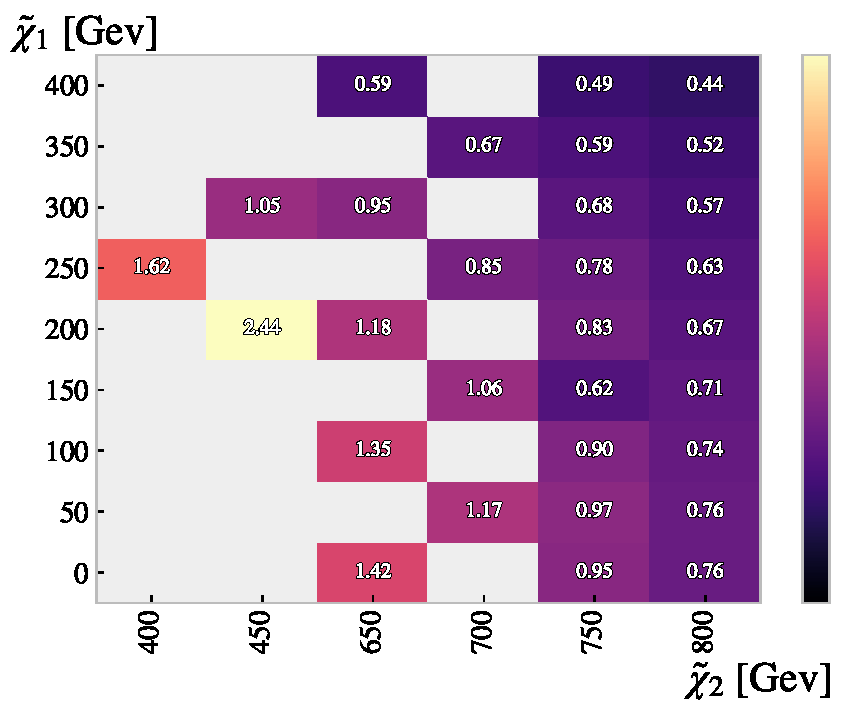
\includegraphics[width=\textwidth]{Figures/MLResults/NN/SUSY/Grid/NNGridSig.pdf}
        \vspace{-1.cm}
        \caption{}
        \label{fig:NNGridSig}
    \end{subfigure}
    }
    \caption{Two grids displaying the expected significance on the original signal set, using the signal region 
    created by two dense \acs{NN}, one with 20 nodes per hidden layer \ref{fig:NNshallowGridSig} and one with 600 \ref{fig:NNGridSig}.}
\end{figure}
\subsection{Parameter Specific Networks and Interpolation}
As I have touched upon in earlier sections, one possible solution to a diverse signal set (in my case a signal set with many 
potential mass combinations) is to implement one model for each individual signal set. Initially one might assume that although 
this approach demands more work, it also produces the strongest performances for all mass combinations individually. I have already 
discussed how, by including different mass combinations in the same data set, we hope to reduce overfitting and potentially allow 
the model to interpolate between the different mass combinations. However, I have not yet discussed how by moving from a one 
mass combination signal set to a diverse set would affect the performance on the original signal. In this section I will present the 
results from an analysis which aims to study this.
\\
In figure \ref{fig:Interpolation} I present the results from two models for which each is trained on two different sets of signals.
The figures display which combinations were used during training, highlighted using a green corner. 
The training performed to produce the results aligns with the strategy described in section \ref{subsec:TrainingStrategy} and both apply
an ordinary dense \ac{NN} architecture described in section \ref{subsec:arch}. Figure \ref{fig:OneMass} presents the achieved sensitivity 
from a dense \ac{NN} which has only trained on one mass combination (which will henceforth be referred to as \ac{OMM}), $\{250,550\}_{GeV}$, 
while figure \ref{fig:SeveralMass} presents the achieved sensitivity after training on a large set of mass combinations 
(which will hence force be referred to as \ac{SMM}). Specifically, the latter figure shows the results after training on all signals on the outer 
square\footnote{I.e. all mass combinations which lie on the edges of the grid.} in the figure \ref{fig:SeveralMass} as well as the point in the 
middle, $\{250,550\}_{GeV}$.\\
\begin{figure}
    \makebox[\linewidth][c]{%
    \centering
    \begin{subfigure}{.6\textwidth}
        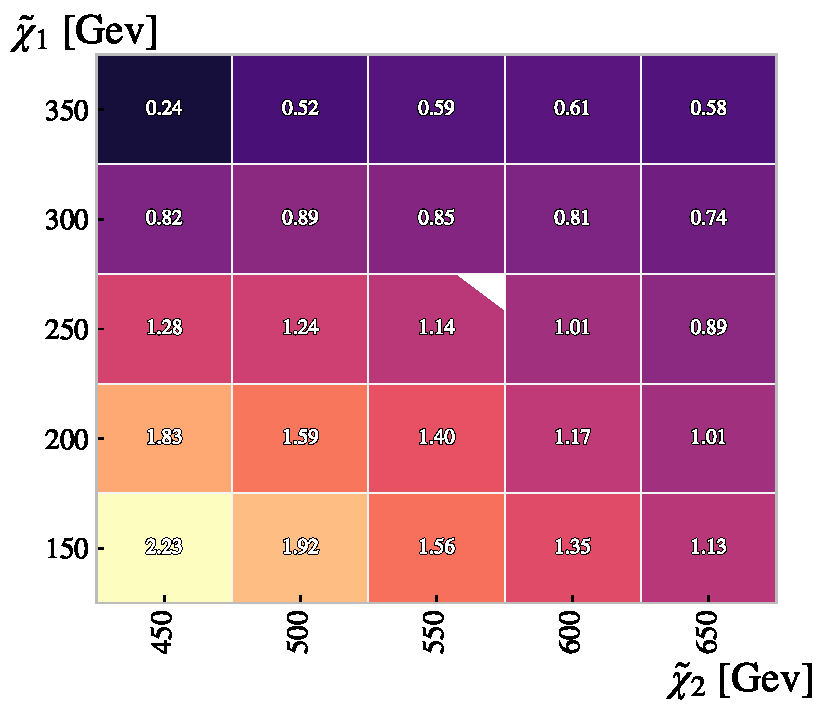
\includegraphics[width=\textwidth]{Figures/MLResults/NN/SUSY/Grid/NN_OneMass_InterpolationGridSig.pdf}
        \vspace{-1.cm}
        \caption{}
        \label{fig:OneMass}
    \end{subfigure}
    \hfill
    \begin{subfigure}{.6\textwidth}
        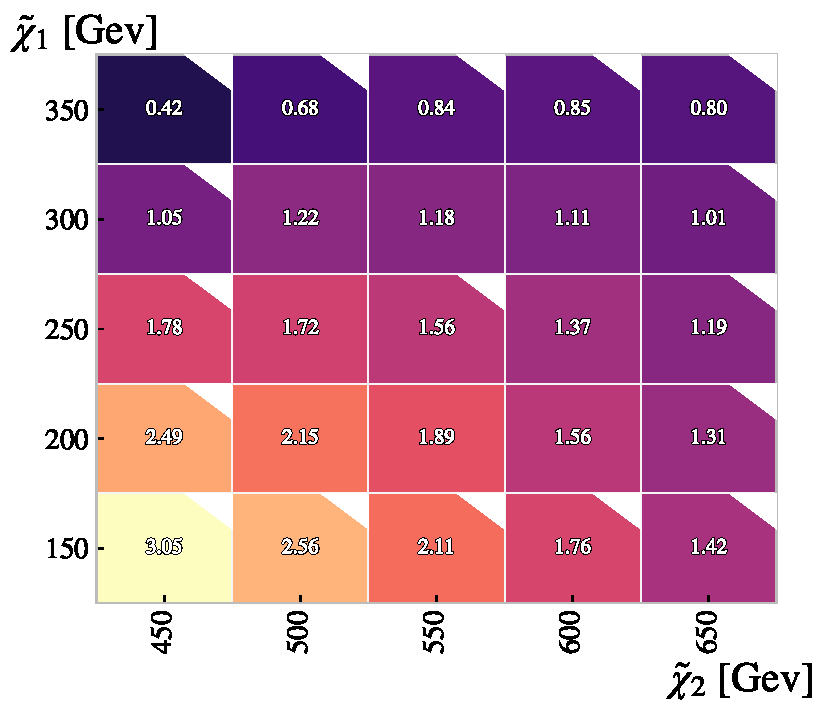
\includegraphics[width=\textwidth]{Figures/MLResults/NN/SUSY/Grid/NN_InterpolationGridSig.pdf}
        \vspace{-1.cm}
        \caption{}
        \label{fig:SeveralMass}
    \end{subfigure}
    }
    \caption[Two grids displaying the expected significance on a subset of the full signal set, using the signal region 
    created by two dense \acs{NN}'s, each training on different amounts of signal.]{Two grids displaying the expected significance 
    on a subset of the full signal set, using the signal region created by two dense \ac{NN}'s. Figure \ref{fig:OneMass} presents the results 
    from a model which has only seen one mass combination during training, $\{250,550\}_{GeV}$. Figure 
    \ref{fig:SeveralMass} presents the results from a model which has seen all mass combinations in the grid, but for the inner square of masses
    around the $\{250,550\}_{GeV}$ point. The figures display which combinations were used during training, highlighted using a green corner. 
    }
    \label{fig:Interpolation}
\end{figure}
My initial prediction for this comparison was that the \ac{OMM} would outperform the \ac{SMM} for the signal with masses
$\{250,550\}_{GeV}$, while underperforming on all other data points. The expectation was that \ac{OMM} 
would learn the trends of the only signal it had seen, while the \ac{SMM} would do the same but for a larger set of mass combinations and 
at the same time interpolate the results for the masses in between. By comparing figures \ref{fig:OneMass} and \ref{fig:SeveralMass} we 
see that my prediction was not completely correct. We can observe that the model which has trained on several-masses outperformed the 
\ac{OMM} on every single combination. At first, I believed this to be caused by the \ac{OMM} overfitting a lot sooner than the other 
model, in other words being stopped earlier in training by the early stopping criteria described in section \ref{subsec:TrainingStrategy}. 
To test this theory, I drew the \ac{AUC} score made after each epoch on both the training and validation set for the \ac{OMM} and the 
\ac{SMM}, shown in Figure \ref{fig:oneMassHist} and \ref{fig:SeveralMassHist}, respectively. By comparing the two figures,
we observe that the \ac{OMM}'s performance on the validation set peaks in the first epoch, therefore stopping training after 
10 epochs, while the \ac{SMM} peaks after 6, allowing the \ac{SMM} model to train longer. This is a clear indication that training on 
one mass combination leads to overfitting. 
\begin{figure}[H]
    \makebox[\linewidth][c]{%
    \centering
    \begin{subfigure}{.45\textwidth}
        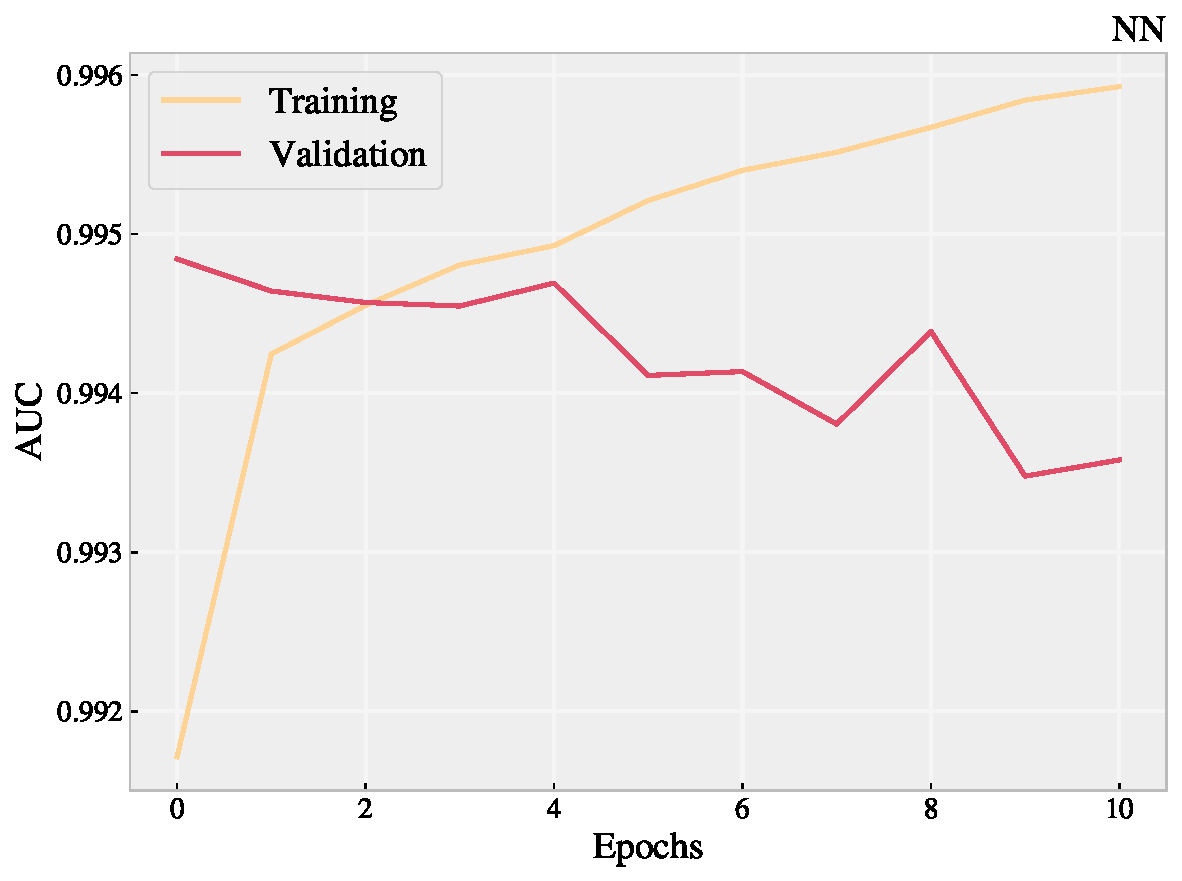
\includegraphics[width=\textwidth]{Figures/MLResults/NN/SUSY/History/NN_OneMass_InterpolationHistory.pdf}
        \caption{}
        \label{fig:oneMassHist}
    \end{subfigure}
    \begin{subfigure}{.45\textwidth}
        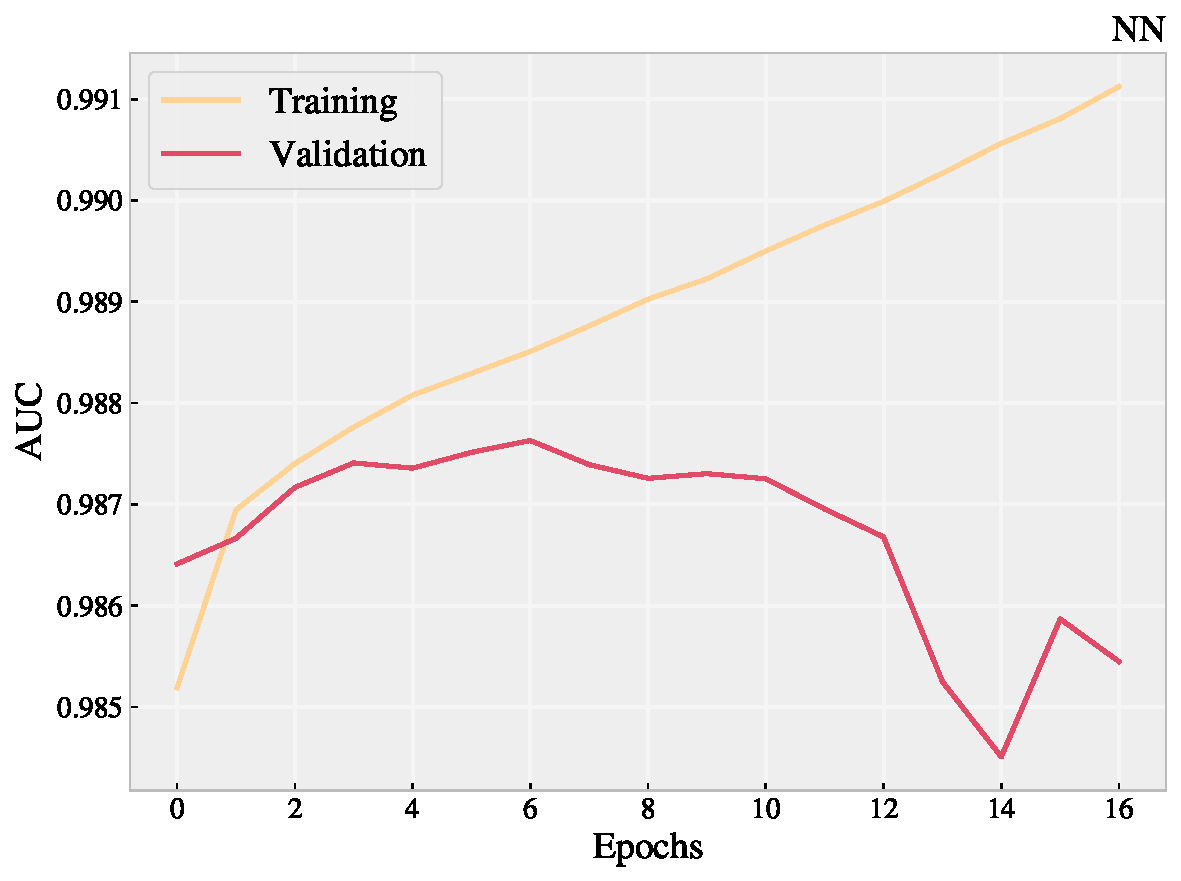
\includegraphics[width=\textwidth]{Figures/MLResults/NN/SUSY/History/NN_InterpolationHistory.pdf}
        \caption{}
        \label{fig:SeveralMassHist}
    \end{subfigure}
    }
    \caption[The comparison of the training history of two \acs{NN}'s, each training on different amounts of signal.]{
    A plot displaying the \acs{AUC} score made after each epoch on both the training and validation set. 
    Figure \ref{fig:oneMassHist} shows the results from the \ac{OMM} and figure \ref{fig:SeveralMassHist} shows
    the results from the \ac{SMM}.}
    \label{fig:InterpolateHistory}
\end{figure}
Given that the \ac{OMM}'s performance is reduced by the early stopping criteria, I wanted to explore if it would be able to outperform the 
\ac{SMM} given it was allowed to train deeper/longer. In figure \ref{fig:NNOverfitting}, I display the achieved significance
of the \ac{OMM} in the case where early stopping has been removed, and the model was allowed to train for 15 epochs. By comparing figures 
\ref{fig:SeveralMass} and \ref{fig:NNOverfitting}, we can observe that even when early stopping is removed from the \ac{OMM}, it is  
still outperformed by the \ac{SMM}. This indicates that overfitting is not the only reason for the \ac{OMM}'s disappointing performance.\\
\begin{figure}[H]
    \centering
    \makebox[\linewidth][c]{%
    \begin{subfigure}{.6\textwidth}
        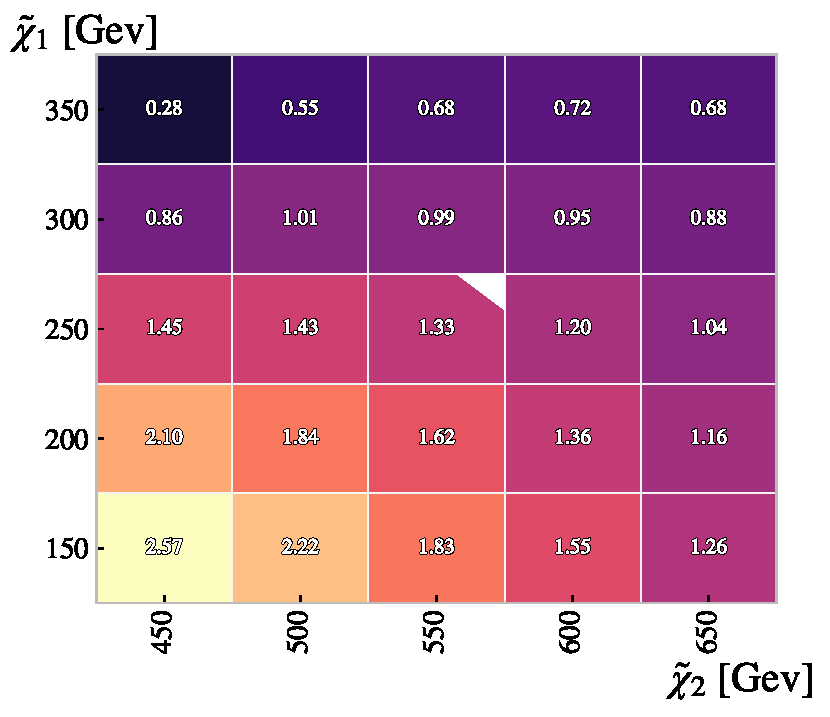
\includegraphics[width=\textwidth]{Figures/MLResults/NN/SUSY/Grid/NN_OneMass_Overfitting15_InterpolationGridSig.pdf}
    \end{subfigure}
    }
    \caption[A grid displaying the expected significance on a subset of the full signal set, using the signal region 
    created by a dense \acs{NN} which has trained on one mass, and has been allowed to train for 16 epochs.]{
    A grid displaying the expected significance on a subset of the full signal set, using the signal region 
    created by the \ac{NN}. The figure presents the results from a model which has only seen one mass combination 
    during training, $\{250,550\}_{GeV}$ and was allowed to train for 15 epochs without 
    early stopping. }
    \label{fig:NNOverfitting}
\end{figure}
The most probable explanation for the underwhelming performance of the \ac{OMM} is that nearby mass combinations (i.e. mass combinations with 
relatively similar masses) exhibit a lot of overlap in terms of feature distributions. In other words, nearby mass combinations (in this example, mass combinations which 
differ by 100GeV) often contribute to the same type of tuning. This means that by including a larger range of signals, which are similar in mass, we are 
essentially increasing the amount of data for each individual signal. This gives further motivation to include diversity in the signal set.